 % !TeX spellcheck = en_US
For a organism to survive, it must be able to perceive and react. Perception includes sensing important elements in the environment -- food, threats, potential mates \dots -- as well as its own state -- energy reserves, damage, disease, \dots -- and must be followed by an integration of the different stimuli into a global picture of the current situation. Thus, food can be ignored when energy reserves are high, but it will become a priority otherwise. The complicated process of sensing, processing information, making decisions and taking action can happen at any level from single cell to a population of multicellular organisms, but it is always based on just a few components that form every single living being. Even if we know this few component make all the work, it would be virtually impossible to figure out, in one single step, which configuration of these components would lead to complex phenomena such as bacterial chemotaxis, nerve impulse transmission or quincea\~nera parties. Natural selection, the artificer of all these phenomena would also be unable to make this combinations in a single step.  The rise of specialized structures, like the brain, is the result of a rearrangement of simpler components that themselves came from the assembly of even simpler ones. In this respect, natural selection has followed a path of ``progress'' very similar to that of any technology. The wheel led to the cart that led to the car and, along the way, we developed traffic lights, air conditioning and microchips. There is a full spectrum of technological complexity that starts with simple components and ends in robots and supercomputers. On the basic side of this complexity spectrum, we find components like resistances, condensers, inductances and transistors, which can be assembled into basic circuits like current and voltage dividers, switches, timers or relays. These circuits can themselves be combined with one another to operate things such as garage doors, escalators and so on. The complexity spectrum of the cell starts with DNA, RNA, membranes and proteins and goes all the way to complex metabolic pathways, organelles and a mobile cytoskeleton. Even though both ends of this spectrum are well studied by biologists, there has been less attention to intermediate combinations, the simpler circuits, and even less to how they can be combined into progressively more complicated molecular machines.

Many critical functions within a cell depend on such circuits and many diseases are the result of failures in their functioning so any attempt at building synthetic biological components or healing these diseases are conditioned by our ability to understand the dynamics of their associated components. In this chapter, we will learn how to combine basic components into the simplest possible circuits and how these circuits are important to achieve different kinds of cellular activity.

\section{Biological circuits}

With biological circuit, we mean a group of biological components (proteins, DNA, RNA, \dots ) that work together to perform a function. To define its behavior, we can say that our circuit is a system that, when confronted with a certain input, will produce a certain output. In biology we often replace the concepts input and output with \textbf{stimulus} and \textbf{response}, respectively.

We are used to talk about electronic circuits by describing their input output response. A doorbell, for instance, has a button that activates a buzzer to make a  a sound while it is pressed. The sound stops when the button is released.  A switch is also a button but, once pressed, it changes to a new state and stays in it. For instance, when we enter a room and press the light switch, the light goes on. After releasing the switch, the light stays on and will only turn off if we press the switch again. From these simple examples we can move on to more complex circuits. A  timer is a circuit that sends a signal after a certain amount of time has passed, a relay is like a switch but it reacts to an electric current instead of physical pressure. We can use relays to open a garage door remotely. Moreover, these simple elements can be combined into a single mechanism: an infra-red sensor can detect the garage remote, send a signal to a relay that opens the garage door -- in technical jargon, an actuator -- and forwards the signal to a timer that waits ninety seconds to  send  the signal back to the relay and
 shut the door. Can we imagine the biological counterparts to these components? Here are some specialized components of the cell that perform critical functions.

\paragraph{Sensors} Cells have many different sensors and some cell types within a body are sensors themselves. We have already mentioned two-component systems in bacteria, which contain sensors able to detect signals out of the cell -- e.g. hormones, food, poisons, \dots -- or in the cell -- levels of acetyl-CoA, osmotic pressure in the membrane, \dots. But there are many more molecules within a cell that can detect signals. Practically every variable that is relevant to cell biology is tracked by one sensor or another: alternative carbon sources can be detected by repressors or activators of the relevant operon, neurotransmitters are detected or imported into post-synaptic neurons  and converted in action potentials, peptidic hormons like insulin are detected by receptors in the surface of the cell while many steroid hormones are imported in the cell where they attach to some protein that binds to DNA \dots 

\paragraph{Signal transduction} The many different signals perceived by the sensors has to be translated to some standard signal. Unlike electronic components, which convert everything to electricity, cellular signals have a wider diversity. A typical mean to transmit signals within the cell is the phosphorylation state of a protein, but other alternatives exist such as methylation states, ion concentrations -- e.g. $K^+$, $Ca^{2+}$, \dots -- or second messengers such as cyclic AMP.
\paragraph{Signal processing} The same signal can trigger different responses in different organisms or even in different cells within the same organism. Liver cells, for instance, respond to insulin by releasing glucose into the bloodstream, while most other cells respond by increasing their glucose uptake. One way of achieving this, is having different components able to respond to a certain signal. Some circuits may show a proportional response to a certain stimulus, others may have an all or nothing response -- e.g. triggering fever when inflammation indicators exceed a certain threshold -- and some systems may behave as a switch, changing their state when a signal is received and staying in this new state. An example of the latter would be cell differentiation, when a signal during embryonic development permanently changes the type of a cell and the genes it expresses.

\paragraph{Other behaviors} The wide diversity of cell behaviors found in nature is proof of the unlimited creativity with which natural selection has been able tweak biological circuits. Molecular clocks keep track of time within the cells and periodic systems, such as those underlying circadian rythms synchronize practically every aspect of our metabolism to the dictates of the  external clock that is sunlight. Some circuits can modify the behavior of sensors. Temperature sensors in the skin of mammals, for instance, do not respond to temperature itself, but rather to changes in it. In other words, the intensity of the signal of a temperature receptor is proportional to the derivative of temperature with respect to time and the same behavior is observed by food receptors governing chemotaxis in bacteria. This type of behavior is called adaptation. 


In this chapter we will see and study several examples of how to build different types of circuits with just a few components. we will build linear transducers, interrupters, switches, oscillators -- clocks-- and circuits able to show adaptation.

\subsection{Linear response}
The simplest possible kind of signal processing is receiving a stimulus ($S$) and transmitting a directly proportional response ($R$) This can be a mean to translate signals -- e.g.  turgor pressure to phosphorylation state, DNA damage to stress protein level, \dots -- or simply to adjust the scale, like in an aplifier. A simple way to build such a system  is depicted in figure \ref{fig:bclin}, where the sythesis of a molecule $R$, is activated by the signal $S$.

\begin{marginfigure}
	\begin{center}
		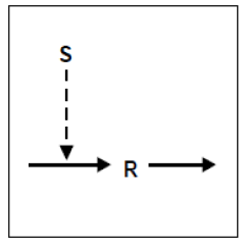
\includegraphics[width=0.9\textwidth]{BiocircLinear}
	\end{center}
	\caption{ ... }
	\label{fig:bclin}
\end{marginfigure}

The equations for this system are:

\begin{equation}
	\frac{dR}{dt}= k_1 \, S - k_2 \, R
\end{equation}

We can solve for the steady state as a function of $S$,
\begin{equation}
	k_1 \, S - k_2 \, R = 0
\end{equation}
and see that the ratio $k_1/k_2$ determines the slope of the stimulus-response curve.

\begin{equation}
	R   = \frac{k_1}{k_2} \, S
\end{equation}

\subsection{Saturated response}
To obtain a saturating stimulus-response curve, we can use a protein that can be phosphorylated by a kinase and dephosphorylated by a phosphatase, where the kinase is activated by $S$. As long as these processes follow linear kinetics, the overall response will be hyperbolic -- saturable.
 
\begin{marginfigure}
	\begin{center}
		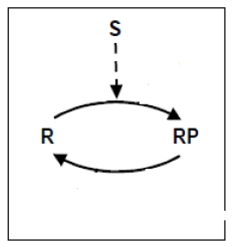
\includegraphics[width=0.9\textwidth]{BiocircMM}
	\end{center}
	\caption{ ... }
	\label{fig:bcsat}
\end{marginfigure}

The equations will be:

\begin{align}
	\frac{dR}{dt} =\:& k_2 \, R_p - k_1 \, S \, R\\
	\frac{dR_p}{dt} =\:& k_1 \, S \, R - k_2 \, R_p	
\end{align}

But The total amount of R protein, $R_T$, is conserved so we can eliminte one equation using the constraint: $R + R_p =R_T$. 

\begin{equation}
	\frac{dR_p}{dt}= k_1 \, S \, \left( R_T-R_p \right ) - k_2 \, R_p
\end{equation}

The steady state condition
\begin{equation}
	k_1 \, S \, \left( R_T-R_p \right ) - k_2 \, R_p = 0
\end{equation}
leads to:
\begin{equation}
	R_p = \frac{k_1 \, S }{k_1 \, S  - k_2} \,  R_T
\end{equation}

Dividing the numerator and the denominator by $k_1$:

\begin{equation}
	R_p = \frac{S}{S  - K_S} \,  R_T
\end{equation}

where $K_S = k_2 / k_1$.

\subsection{Sigmoidal response}
S-shaped curves are ubiquitous in biology. Allosteric enzymes and proteins, such as hemoglobin, show this kind of response, and so do many transcription factors. Sigmoidal stimulus-response curves approximate an all or nothing transition once the stimulus passes a certain threshold. They are the biological equivalents of the doorbell with a buzzer.

\begin{marginfigure}
	\begin{center}
		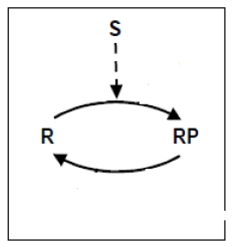
\includegraphics[width=0.9\textwidth]{BiocircMM}
	\end{center}
	\caption{ ... }
	\label{fig:bcsigmoid}
\end{marginfigure}


\subsection{Switch}
Switches also provide all or nithing type transitions but they bring a totally new, and very important property to the table, memory. A switch maybe very similar in its stimulus response curve when we activate it. When $S$ increases  past the threshold, a switch transitions from  very low  to very high levels of $R_p$. When the stimulus disappears, however, the switch will stay at the activated state -- high $R$ -- so it remembers its state and reserves it. This ability is obviously very important for some biological processes such as cell differentiation, where a signal during the embryonic stage determines the type of a cell --neuron, adipocyte, leucocyte, \dots -- for the rest of the life on an individual.

Switch-like behavior is based on a property called bistability, that manifests itself when a system has two stable steady states. It is noteworthy that bistability requires three steady states, two stable and one unstable, that acts as a barrier between the others.

A very simple system with this behavior can be built with a single state variable that will stay in whichever state it is set. This kind of self-switching behavior is typical for cases like the lambda phage, which can alternate between lytic and lysogenic modes of operation. The same behaviour would be observed by any protein able to activate its own expression.

\begin{marginfigure}
	\begin{center}
		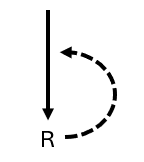
\includegraphics[width=0.9\textwidth]{bistab}
	\end{center}
	\caption{ ... }
	\label{fig:bistab}
\end{marginfigure}

equations:

\begin{equation}
	\frac{dR}{dt} = \beta + \alpha \frac{R^n}{R^n  + K_R^n} - k_d \, R
\end{equation}

With the first two terms being constitutive and inducible synthesis respectively and the negative term accounting for degradation and possibly dillution.

The presence of the three steady states can be easily seen graphically by plotting overall synthesis and degradation as functions of $R$. Figure \ref{fig:bistabkin} shows how this system may have three different steady states.

\begin{figure}
	\begin{center}
		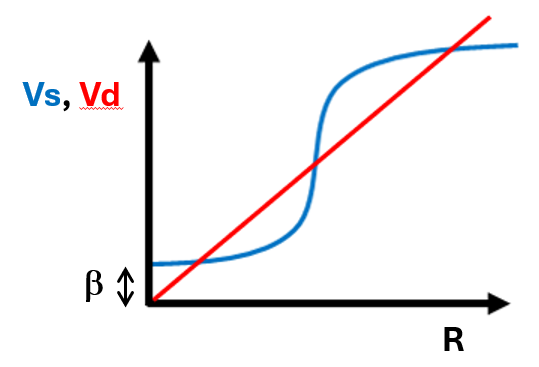
\includegraphics[width=0.7
		\textwidth]{bistabkinetics}
	\end{center}
	\caption{ ... }
	\label{fig:bistabkin}
\end{figure}

The steady states could be calculated from the equation:

\begin{equation}
	 \beta + \alpha \frac{R^n}{R^n  + K_R^n} - k_d \, R = 0
\end{equation}

Instead of calculating all three steady states exactly, we will take advantage of this situation to work with approximations. Lets calculate the low steady state assuming $| R |_1 << K_R$, then the inducible term will be negligible and the system will behave as

\begin{equation}
	\frac{dR}{dt} \approx \beta - k_d \, R
\end{equation}

with the steady state

\begin{equation}
	|R|_1 \approx \frac{\beta}{k_d }
\end{equation}

and the linearized system will be:

\begin{equation}
	\frac{d}{dt} \delta R =  - k_d \, \delta R
\end{equation}

with solution $\delta R = k \, e^{- k_d\, t}$, so it will be stable.

For the high value $| R |_3 >> K_R$,


\begin{equation}
	\frac{R^n}{R^n  + K_R^n}  \approx 1
\end{equation}

\begin{equation}
	\frac{dR}{dt} \approx \beta + \alpha - k_d \, R
	\label{stab_st_autoinduce}
\end{equation}


\begin{equation}
	|R|_3 \approx \frac{\alpha + \beta}{k_d }
\end{equation}

And the linearized system will also be equation  \ref{stab_st_autoinduce}, so it is stable as well.

Now for the middle state we know $|R|_1 \leq |R|_2 \leq |R|_3$ and we can make the dubious assumption $|R|_2 \approx K_R$. Tempted as we may be to just assume that the inducible term will be $\alpha/2$, we cannot neglect the dependency of this term on $R$ itself \dots

% a ver como salgo de este jardin

\subsection{Oscillators (clocks)}
\subsection{Adaptation}

\begin{marginfigure}
	\begin{center}
		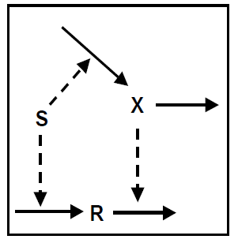
\includegraphics[width=0.9\textwidth]{BiocircAdapt}
	\end{center}
	\caption{ ... }
	\label{fig:bcadapt}
\end{marginfigure}

\subsection{Quorum sensing}